\noindent \textred{1.} 
Assume that the DFS procedure considers (explores) the vertices in alphabetical order, and assume the adjacency list is ordered alphabetically.
\begin{itemize}
    \item[(a)] Run TOPOLOGICAL-SORT on Fig.\ref{fig:Q1-a}. Show:
    \begin{itemize}
        \item[i.] the discovery time and finish time of each node;\\
        \myAnswer{
        The discover time and the finish time are denoted with \textgreen{green} numbers and \textred{red} numbers respectively in Fig.\ref{fig:Q1-a}.
        }
        \item[ii.] the returned linked-list. \\
        \myAnswer{
        $\{p, n, o, s, m, x, r, y, v, w, z, u, q, t\}$
        }
    \end{itemize}
\begin{figure}[!h]
    \centering
    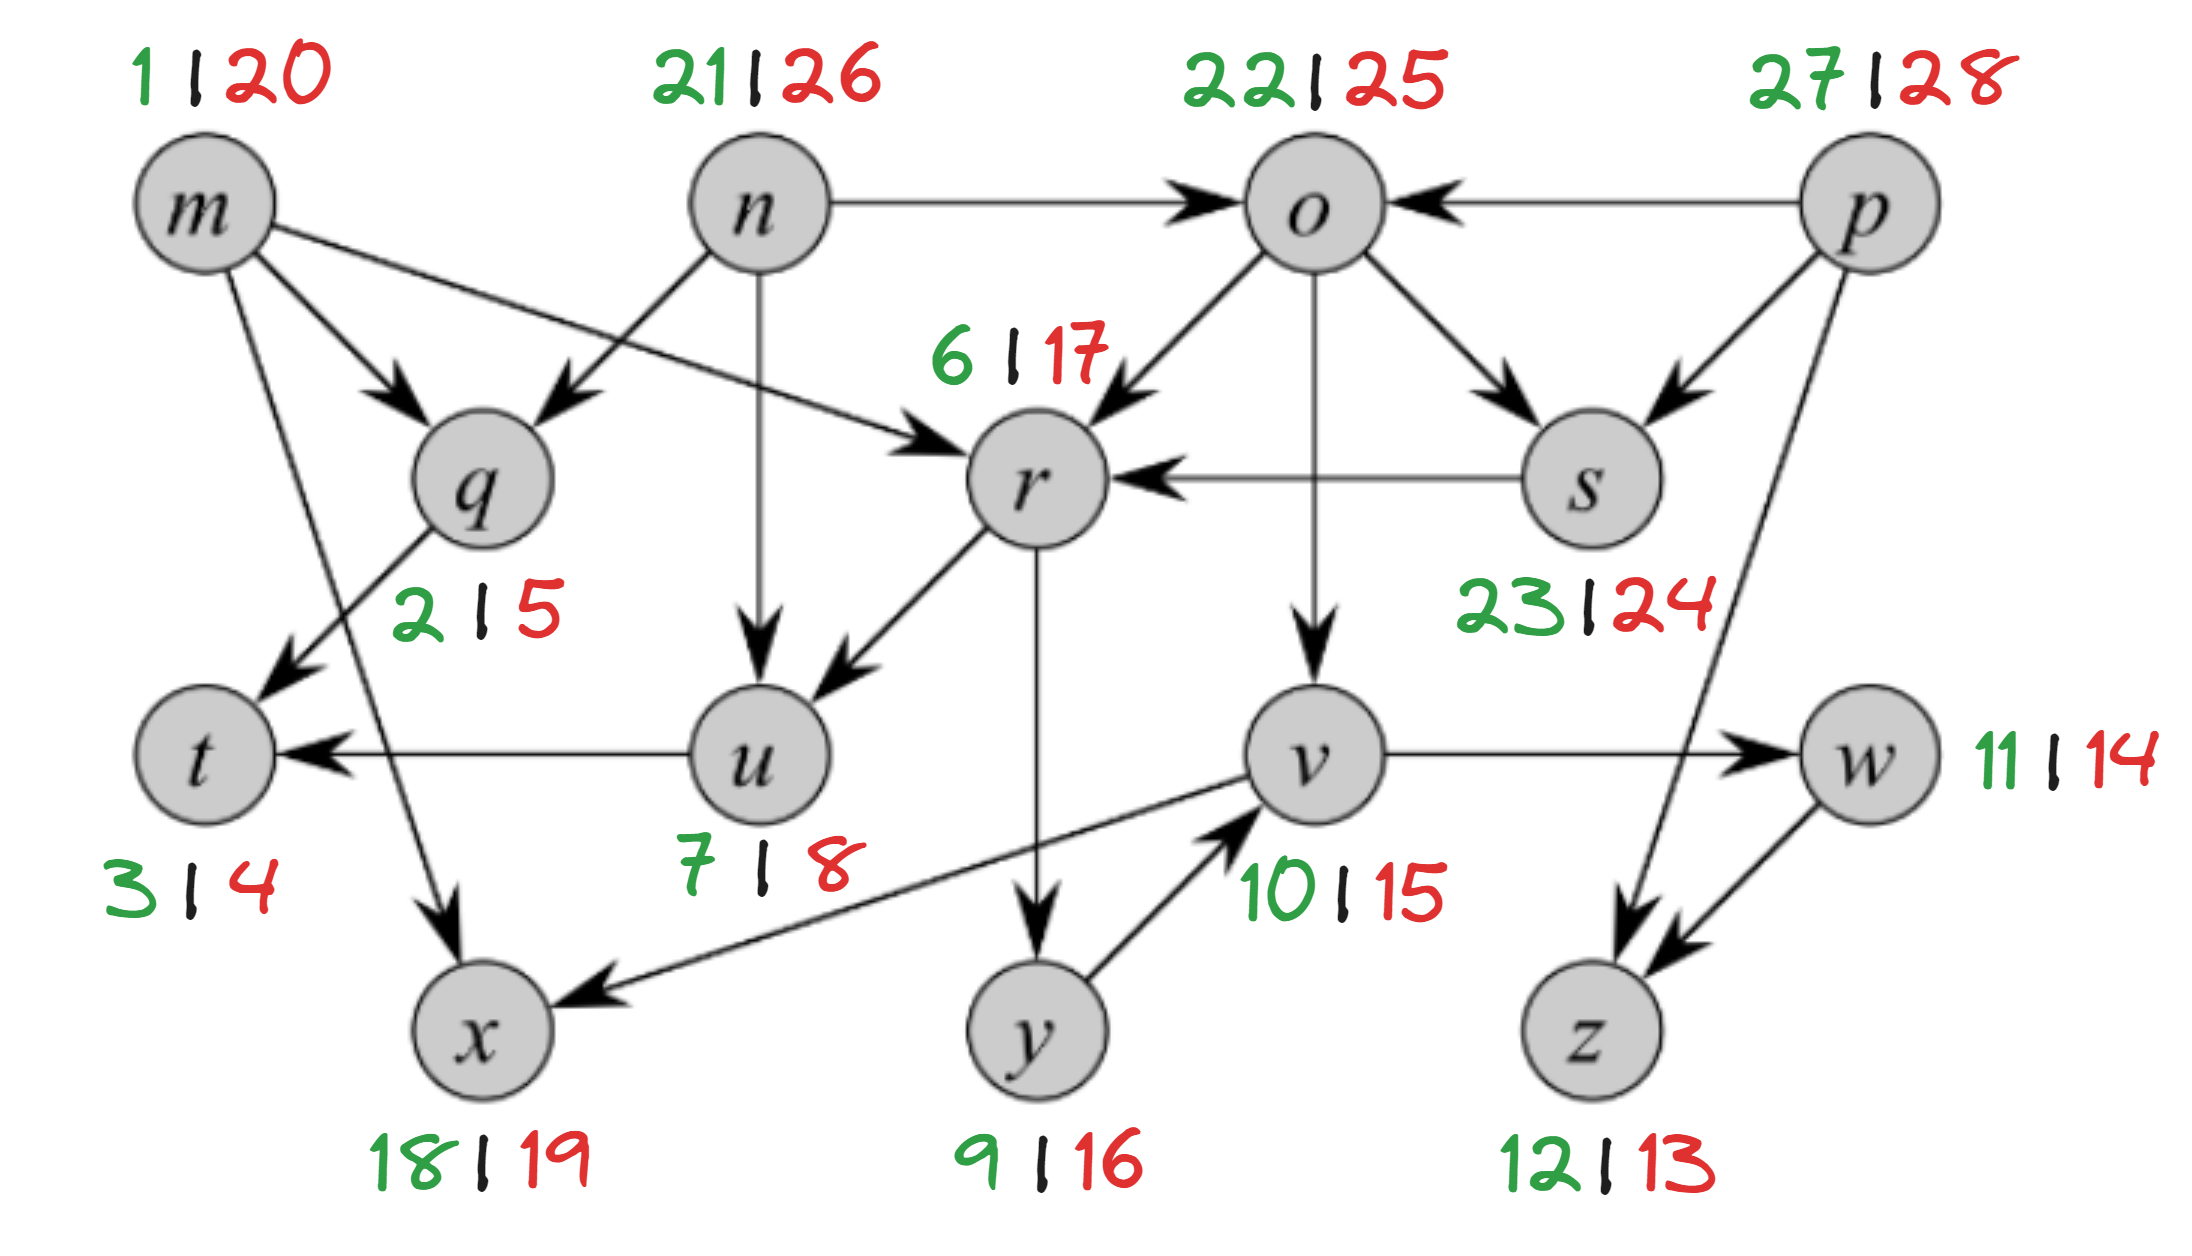
\includegraphics[width=0.65\linewidth]{HWs//HW9//figures/1-1-my.png}
    \caption{Graph for Q1(a)}
    \label{fig:Q1-a}
\end{figure}
    \item[(b)] Run STRONGLY-CONNECTED-COMPONENTS on Fig.\ref{fig:Q1-b}. Show:
    \begin{itemize}
        \item[i.] The discovery time and finish time for each node after running the first-pass DFS;\\
        \myAnswer{
        The discover time and the finish time are denoted with \textgreen{green} numbers and \textred{red} numbers respectively in Fig.\ref{fig:1-2-1}.
        }
        \item[ii.] The discovery and finish time for each node in the second-pass DFS on the transposed graph;\\
        \myAnswer{
        The discover time and the finish time are denoted with \textgreen{green} numbers and \textred{red} numbers respectively in Fig.\ref{fig:1-2-2}.
        }
        \item[iii.] The DFS forest produced by the second-pass, and the component DAG.\\
        \myAnswer{
        The DFS forest has been denoted with blue circles in Fig.\ref{fig:1-2-2}, and the component DAG is shown in Fig.\ref{fig:1-2-3}.
        }
    \end{itemize}
\end{itemize}
\newpage
\begin{figure}[!ht]
    \centering
    \begin{subfigure}[b]{\textwidth}
         \centering
         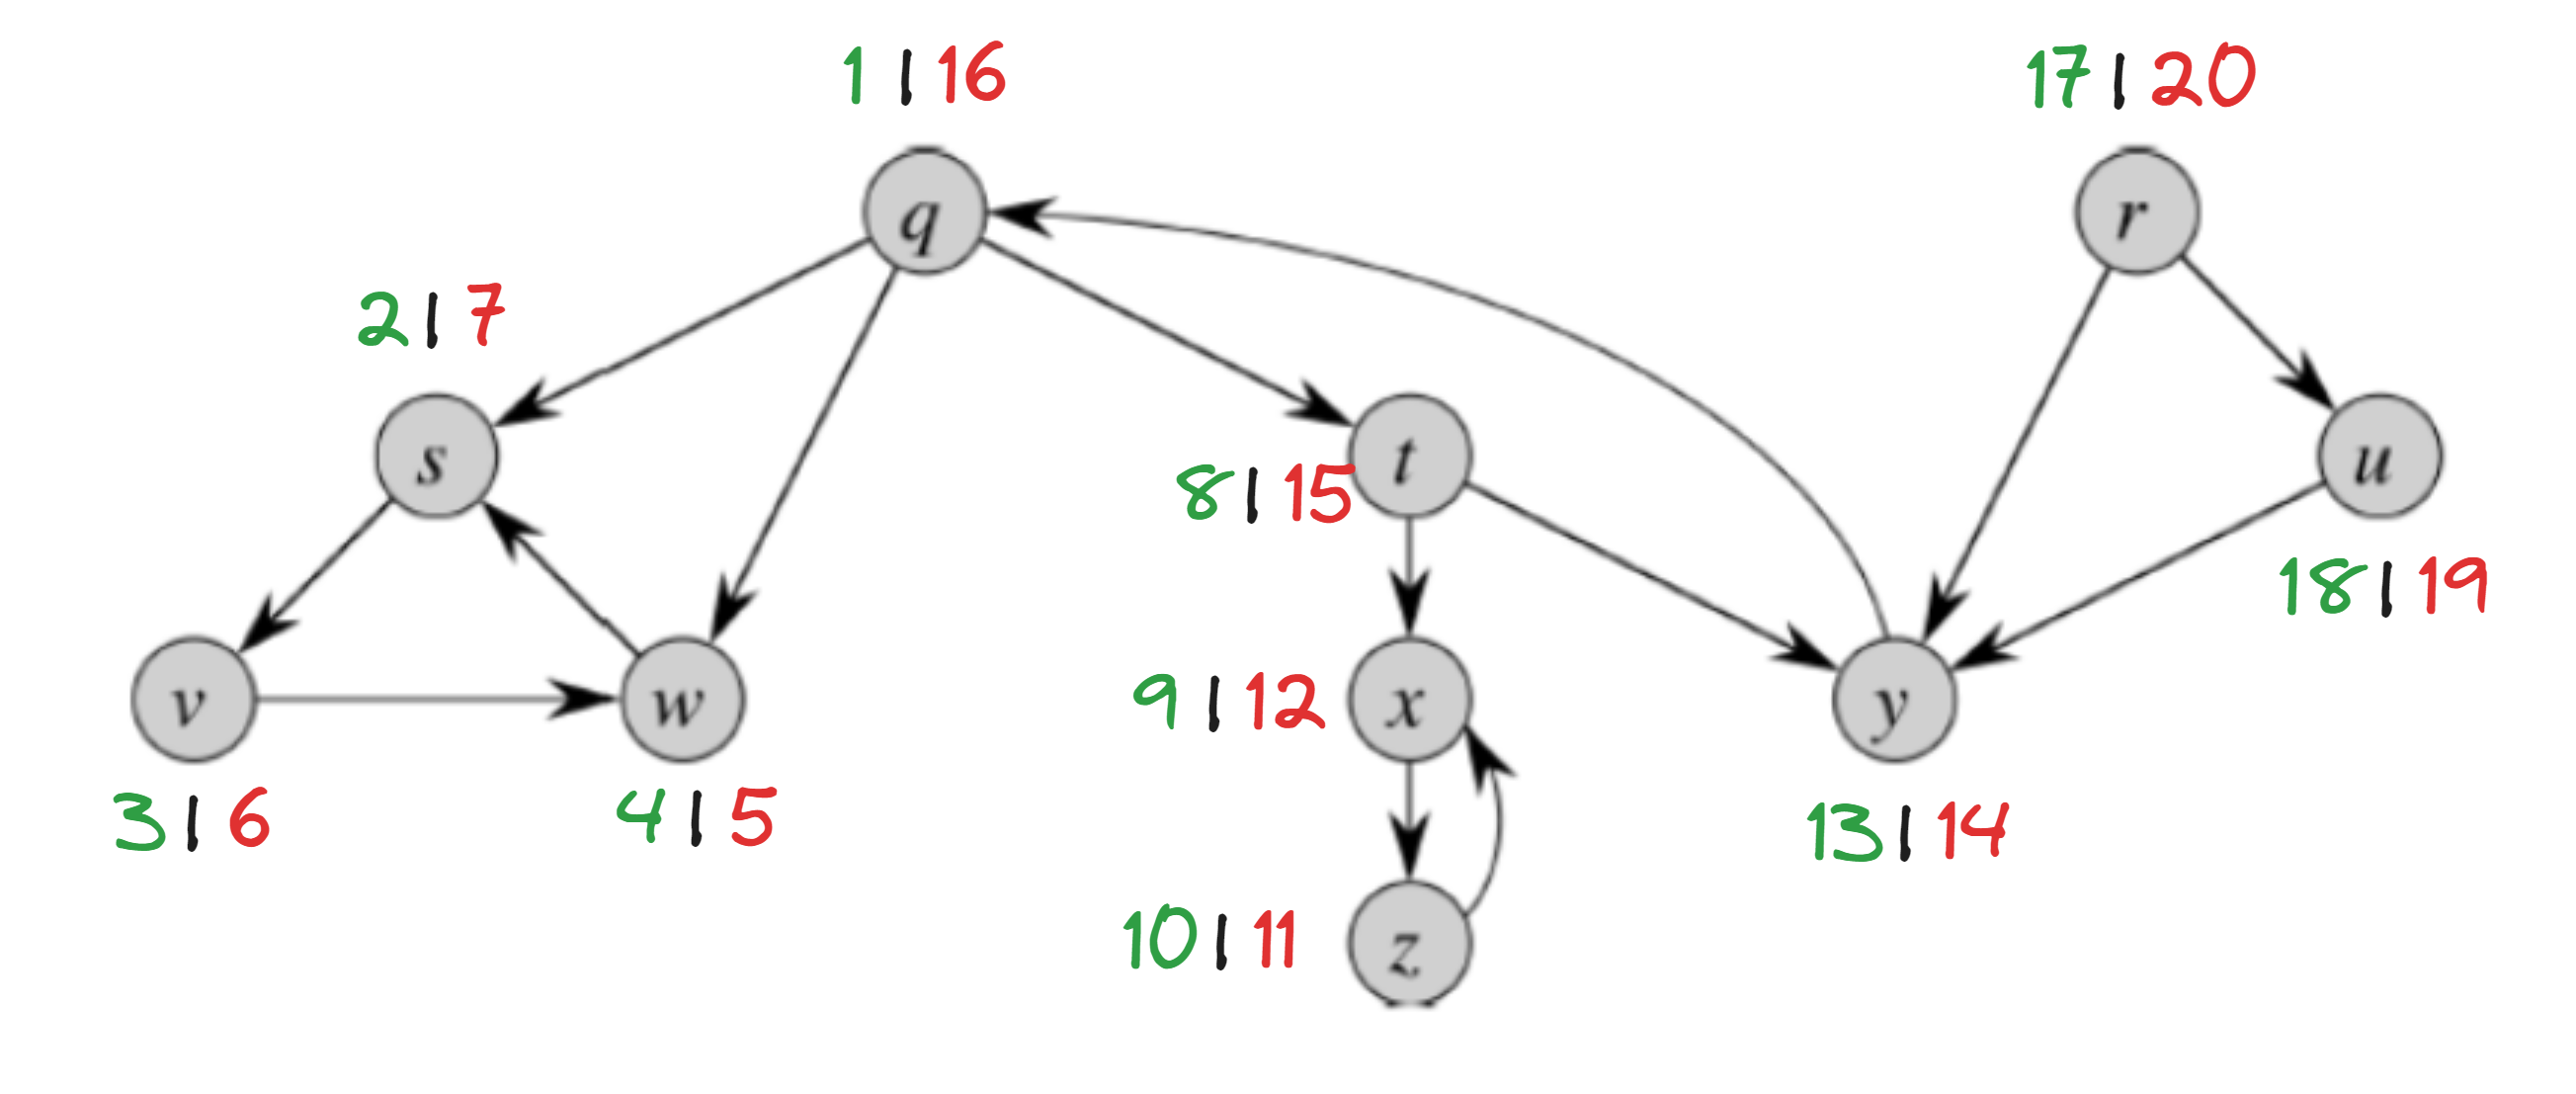
\includegraphics[width=0.75\linewidth]{HWs//HW9//figures/1-2-1.png}
         \caption{first-pass on $G$}
         \label{fig:1-2-1}
    \end{subfigure}
    \begin{subfigure}[b]{\textwidth}
         \centering
         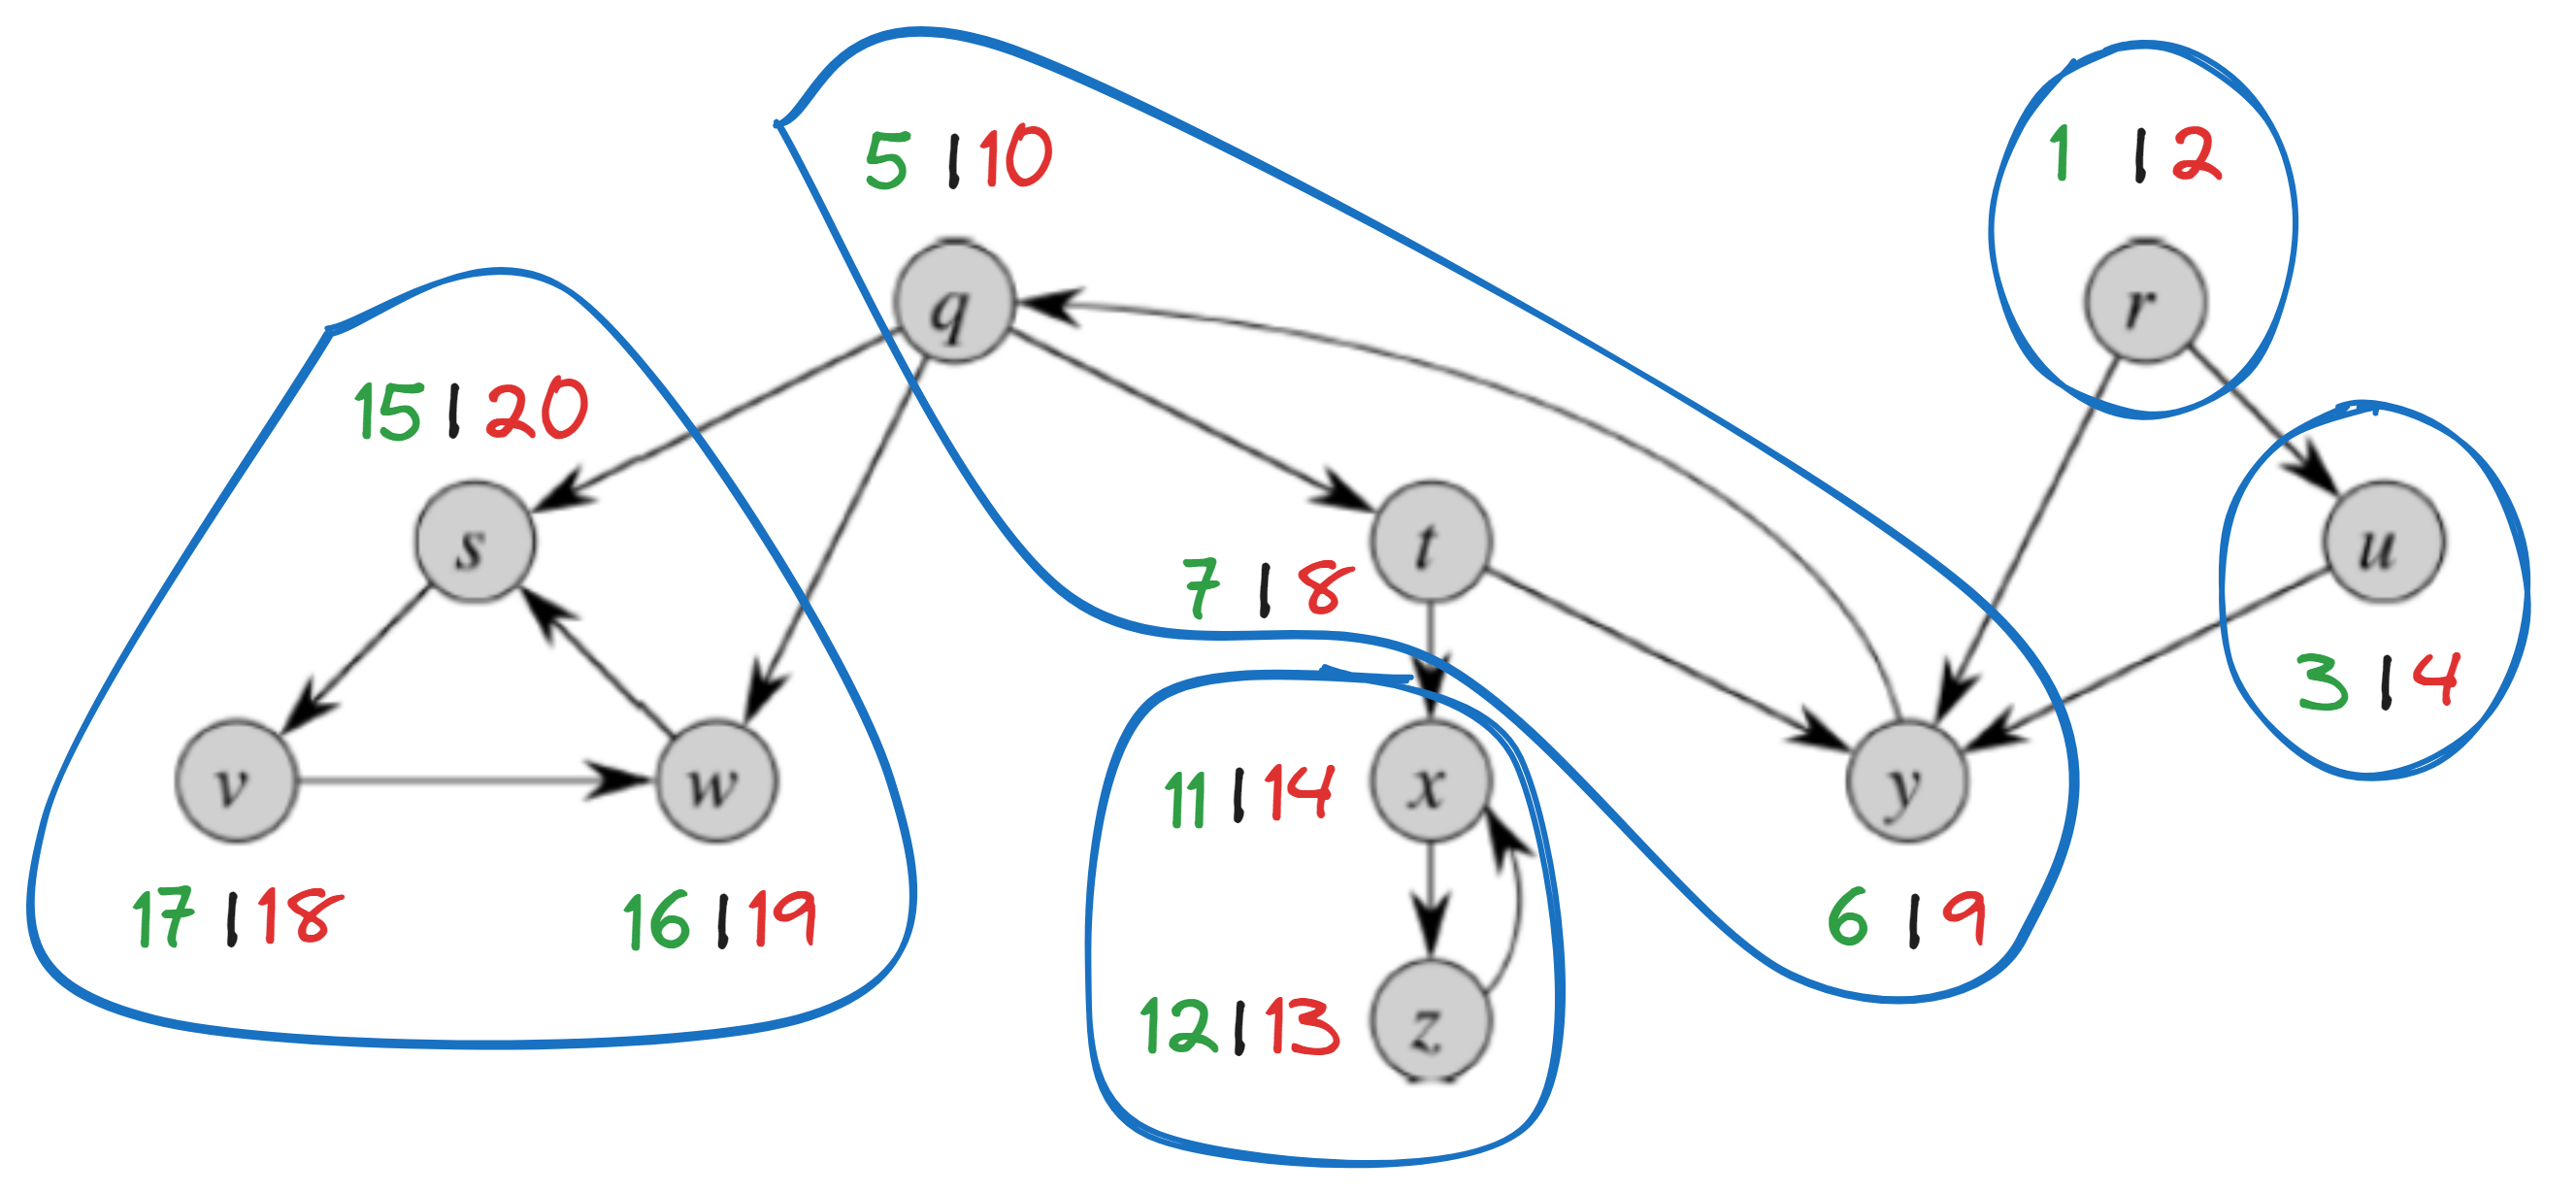
\includegraphics[width=0.75\linewidth]{HWs//HW9//figures/1-2-2.png}
         \caption{second-pass on $G^T$}
         \label{fig:1-2-2}
    \end{subfigure}
    \begin{subfigure}[b]{\textwidth}
         \centering
         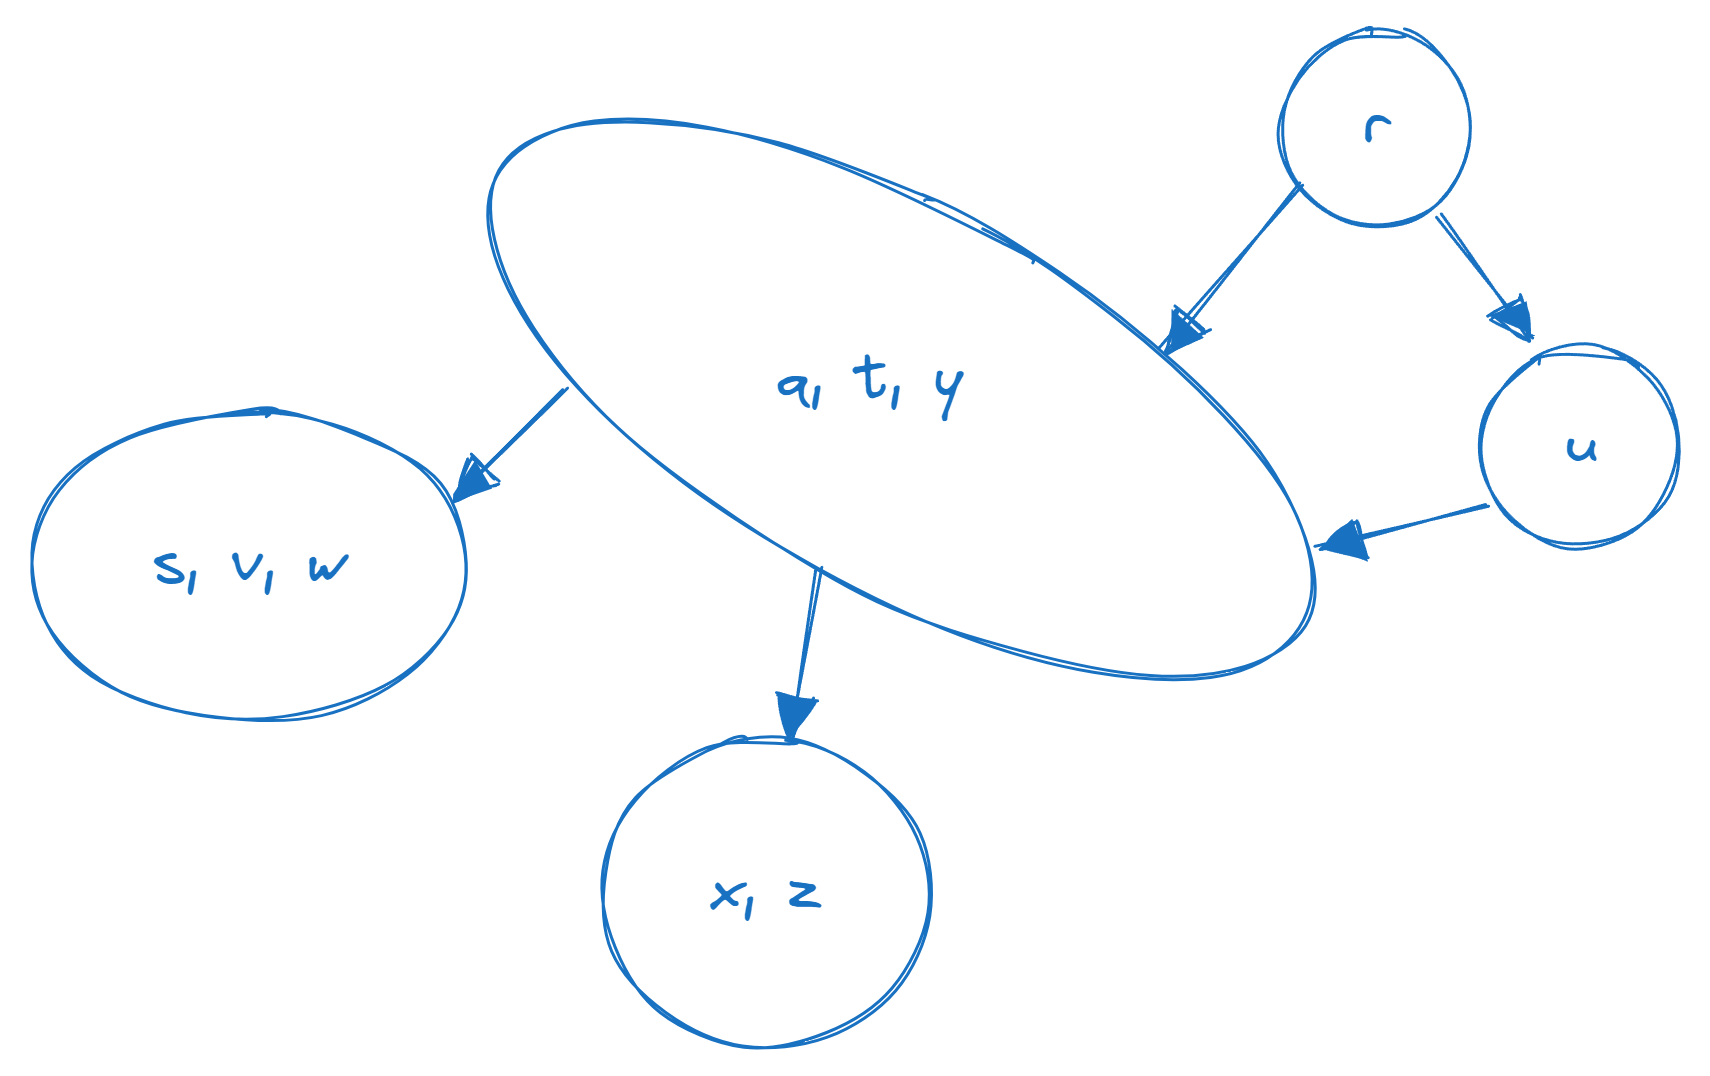
\includegraphics[width=0.6\linewidth]{HWs//HW9//figures/1-2-3.png}
         \caption{component DAG}
         \label{fig:1-2-3}
    \end{subfigure}
    \caption{Graph for Q1(b)}
    \label{fig:Q1-b}
\end{figure}
